% Capítulo 10: captura por valor (cópia) e por referência em uma lambda.
\documentclass[border=4pt]{standalone}
\usepackage[utf8]{inputenc}
\usepackage[T1]{fontenc}
% Estilo comum das figuras de vetores (capítulo 8).
\usepackage{tikz}
\usetikzlibrary{arrows.meta, positioning, calc, decorations.pathreplacing}
\definecolor{navy}{RGB}{23,45,80}
\definecolor{laranja}{RGB}{250,110,29}
\definecolor{cinzalogo}{RGB}{107,114,126}
\definecolor{azul}{RGB}{205,222,247}
\tikzset{
  casa/.style={draw=navy, line width=0.9pt, minimum width=8mm, minimum height=7mm,
               inner sep=0pt, font=\sffamily\small},
  pronta/.style={casa, fill=azul},
  parte/.style={casa, fill=laranja!12},
  marcada/.style={casa, fill=laranja!45, draw=laranja},
  fora/.style={casa, draw=cinzalogo!60, dashed, fill=white, text=cinzalogo!60},
  indice/.style={font=\sffamily\scriptsize, text=cinzalogo},
  explica/.style={font=\sffamily\small, text=navy, anchor=east},
  legenda/.style={font=\sffamily\scriptsize, text=cinzalogo},
  rotulo/.style={font=\sffamily\small\bfseries, text=navy},
  seta/.style={-{Stealth[length=2.2mm]}, navy, line width=0.9pt},
  chave/.style={decorate, decoration={brace, amplitude=4pt, mirror}, navy, line width=0.8pt},
}
% \vetor{nome}{x}{y}{valor/estilo, valor/estilo, ...}: casas lado a lado, chamadas nome0, nome1...
\newcommand{\vetor}[4]{%
  \foreach \valor/\estilo [count=\i from 0] in {#4} {
    \node[\estilo] (#1\i) at ($(#2, #3) + (\i*0.8, 0)$) {\valor};
  }
}

\tikzset{
  caixa/.style={draw=navy, line width=0.9pt, rounded corners=2pt, minimum width=30mm,
                minimum height=9mm, font=\ttfamily\small, align=center},
  variavel/.style={caixa, fill=laranja!12},
  lambda/.style={caixa, fill=azul},
  titulo/.style={font=\sffamily\small\bfseries, text=navy},
}
\begin{document}
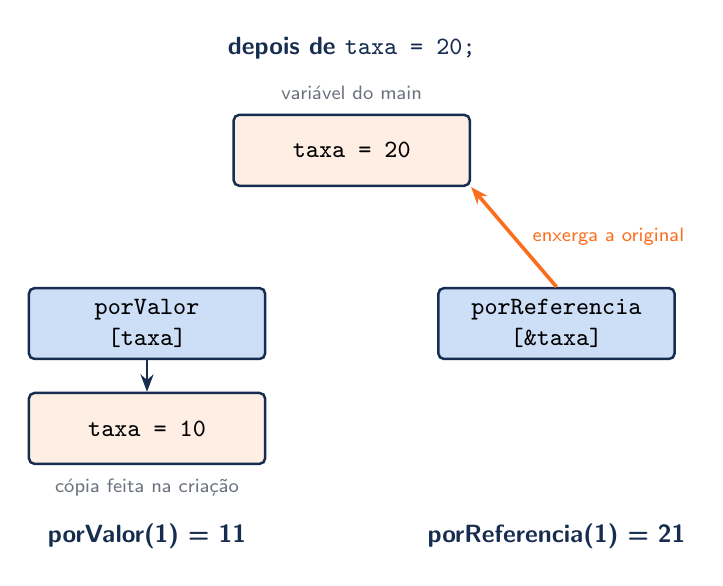
\begin{tikzpicture}
  \node[titulo] at (2.6, 1.3) {depois de \texttt{taxa = 20;}};
  \node[variavel] (taxa) at (2.6, 0) {taxa = 20};
  \node[legenda, above=0.5mm of taxa] {variável do main};

  \node[lambda] (valor) at (0, -2.2) {porValor\\{[taxa]}};
  \node[variavel, below=4mm of valor] (copia) {taxa = 10};
  \node[legenda, below=0.5mm of copia] {cópia feita na criação};
  \draw[seta] (valor) -- (copia);

  \node[lambda] (ref) at (5.2, -2.2) {porReferencia\\{[\&taxa]}};
  \draw[seta, laranja, line width=1.3pt] (ref.north) -- node[legenda, text=laranja, right=1mm] {enxerga a original} (taxa.south east);

  \node[rotulo] at (0, -4.9) {porValor(1) = 11};
  \node[rotulo] at (5.2, -4.9) {porReferencia(1) = 21};
\end{tikzpicture}
\end{document}
